
\documentclass[a4paper,12pt,fleqn]{article}
\usepackage{amsfonts}
\usepackage{amsthm}
\usepackage{graphicx}

\setlength{\parindent}{3em}
\setlength{\oddsidemargin}{0in}
\setlength{\textwidth}{6.5in} % sets 1in left and right margins
\setlength{\topmargin}{0.0in} % change to 0.2in for regular latex
%\setlength{\headheight}{0in}
%\setlength{\footheight}{0.5in}
\setlength{\footskip}{0.5in}
\setlength{\textheight}{9.0in} %sets 1in top and bottom margins
%\renewcommand{\baselinestretch}{1} %set to 1.5 for double spacing.


\newtheorem{Prop}{Proposition}
\newtheorem{lemma}{Lemma}

\newcommand{\br}{{\mathbf r}}
\newcommand{\bA}{{\mathbf A}}
\newcommand{\ba}{{\bf a}}
\newcommand{\bb}{{\bf b}}
\newcommand{\bc}{{\bf c}}
\newcommand{\bC}{{\bf C}}
\newcommand{\bd}{{\bf d}}
\newcommand{\be}{{\bf e}}
\newcommand{\bq}{{\bf q}}
\newcommand{\bs}{{\bf s}}
\newcommand{\bn}{{\bf n}}
\newcommand{\bm}{{\bf m}}
\newcommand{\bu}{{\bf u}}
\newcommand{\bv}{{\bf v}}
\newcommand{\bw}{{\bf w}}
\newcommand{\bx}{{\bf x}}
\newcommand{\bbf}{{\bf f}}
\newcommand{\bL}{{\bf L}}
\newcommand{\bM}{{\bf M}}
\newcommand{\bN}{{\bf N}}
\newcommand{\bS}{{\bf S}}
\newcommand{\bT}{{\bf T}}
\newcommand{\bD}{{\bf D}}
\newcommand{\bX}{{\bf X}}
\newcommand{\bP}{{\bf P}}
\newcommand{\bQ}{{\bf Q}}
\newcommand{\bI}{{\bf I}}
\newcommand{\bR}{{\bf R}}
\newcommand{\bU}{{\bf U}}
\newcommand{\bV}{{\bf V}}
\newcommand{\bW}{{\bf W}}
\newcommand{\bJ}{{\bf J}}
\newcommand{\bB}{{\bf B}}
\newcommand{\bzero}{{\bf 0}}
\newcommand{\bgamma}{{\mbox {\boldmath $\gamma$}}}
\newcommand{\btheta}{{\mbox {\boldmath $\theta$}}}
\newcommand{\bLambda}{{\mbox {\boldmath $\Lambda$}}}
\newcommand{\bPsi}{{\mbox {\boldmath $\Psi$}}}
\newcommand{\bPhi}{{\mbox {\boldmath $\Phi$}}}
\newcommand{\bcS}{{\mbox {\boldmath ${\cal S}$}}}
\newcommand{\bcH}{{\mbox {\boldmath ${\cal H}$}}}
\newcommand{\bcI}{{\mbox {\boldmath ${\cal I}$}}}
\newcommand{\bcR}{{\mbox {\boldmath ${\cal R}$}}}
\newcommand{\bcB}{{\mbox {\boldmath ${\cal B}$}}}

\title{ On Soft Interference Cancellation for Synchronous CDMA}
\date{}
\author{ Shu Wang, James Caffery, Jr. and Hanhong Shen\\ ECE\&CS Department\\ University of Cincinnati \\Cincinnati, OH 45211-0030}
\begin{document}
\maketitle

\begin{abstract}
Compensating for near-far effects is critical for satisfactory
performance of Code Division Multiple Access (CDMA) systems.
Interference cancellation is one of the multiuser detection (MUD)
methods for suppressing the effects from the multiple access
interference (MAI) and consequently improving the system
performance. In this paper, the principles of interference
cancellation (IC) for synchronous CDMA are reviewed. We introduce
several soft interference cancellation schemes, including
individually and jointly optimum interference cancellation, direct
interference cancellation, maximum asymptotic multiuser efficiency
(MAME) interference cancellation and minimum mean-square error
(MMSE) interference cancellation algorithms. In addition to
showing that optimum multiuser detection and MAME multiuser
detection can be realized as interference cancellers, the direct
interference cancellation detector can be taken as the special
realization of the classic decorrelating detection while the
linear MMSE interference cancellation has the same performance as
the linear MMSE multiuser detector.
\end{abstract}

\section{Introduction}

Direct-sequence code division multiple access (DS/CDMA) techniques
have attracted increasing attention for efficient use of available
bandwidth, resistance to interference and flexibility to variable
traffic patterns. Multiuser detection strategy is a method to
minimize the effects of MAI and mitigate the near-far problem in
CDMA systems. It has been extensively investigated over the past
several years~\cite{Verd98}, since MAI is the dominant impairment
for CDMA systems and exists even with perfect power control. Since
1980s, there have been lots of work conducted on the derivation
and analysis of the optimum multiuser receivers. The optimum
multiuser receiver was developed by
Verd\'{u}~\cite{Verd83a,Verd83b,Verd84}, but has overwhelming
complexity. The large gaps in performance and complexity between
the conventional single-user matched filter and optimum multiuser
detector encouraged the search for other multiuser detectors that
exhibit good performance/complexity tradeoffs. There has been
considerable interest in linear multiuser detection based on
decorrelating, MAME or MMSE
criterion~\cite{Lupa89,Lupa90,Madhow94}.

The classic decorrelating detector~\cite{Lupa89} not only is a
simple and natural strategy but also is optimal according to three
different criteria: least squares, near-far
resistance~\cite{Verd86} and maximum-likelihood when the received
amplitudes are unknown~\cite{Lupa89}. Linear multiuser detectors
can be implemented in a decentralized fashion where only the
user(s) of interest need be demodulated. In the MAME linear
multiuser detector~\cite{Lupa90}, the computational complexity is
prohibitive for large number of user. For MMSE linear multiuser
detector~\cite{Madhow94}, although it doesn't achieve minimum
bit-error rate (BER), it has been proved to achieve optimal
near-far resistance. It is shown that there is no explicit
knowledge of interference parameters required in MMSE detector.
More recently, it suggested that the output of MMSE detector can
be accurately approximated by Gaussian noise in many
cases~\cite{Poor97a}. Compared to decorrelating detector and MAME
detector, MMSE detector can be blindly realized without any
knowledge of interference parameters.

Interference
cancellation~\cite{Yoon93,Patel94,Wijk95,Divsalar96,Kim98,Bugallo01}
provides a promising alternative to the conventional or optimum
detectors in multiuser detection. Interference cancellation
methods typically require less implementation complexity while
practically offering similar performance. The idea behind
interference cancellation is to estimate the multiple access
and/or multipath induced interference and then to subtract the
interference estimate from the received signal. Hence, compared to
other multiuser detection schemes, interference cancellation pays
more attention on the estimation of the MAI. Different schemes for
the MAI estimation lead to different interference cancellation
schemes. Actually, interference cancellation detector will cancel
the interfering signal exactly provided that the decision was
correct and channel information is known. Otherwise it will double
the contribution of the interferers. The main alternatives for
implementation of interference cancellation are parallel hard
interference cancellation (PIC) and serial/successive hard
interference cancellation (SIC)~\cite{Patel94,Wijk95}, while many
other variants on these basic principles have also been developed.
With conventional PIC~\cite{Divsalar96,Kim98}, all user are
simultaneously demodulated and detected in a parallel behave. With
conventional SIC, a decision for the symbol of the stronger user
is made first, the interference from this user is subsequently
removed in the the next stronger user's receiver before the next
user's receiver make its decision and so on.

In this work, we consider a synchronous DS/CDMA system and review
the principles of interference cancellation. several soft
interference cancellation schemes, including individually and
jointly optimum interference cancellation, direct interference
cancellation detector, MAME interference cancellation detector and
MMSE interference detector, are introduced with different MAI
estimation schemes. With the discussion of the relationship
between soft interference cancellation and multiuser detection, we
show that, besides optimum interference cancellation and MAME
interefence cancellation, the proposed direct interference
cancellation detector has the same performance of the classic
decorrelating detector while the MMSE multiuser detection and the
MMSE interference cancellation actually are the same detectors.

The rest of the paper is organized as follows. In Section II, we
summarize the signal model. In Section III, we review the
interference cancellation in multiuser detection and proposed the
direct interference cancellation, maximum asymptotic multiuser
efficiency interference cancellation and minimum mean-square error
interference cancellation detectors, besides those optimum
interference cancellations. In Section IV, some theoretical
analysis results are present. In section V, the conclusion are
presented, respectively.

\section{Data Model and Problem Description}

The basic CDMA $K$-user channel model, consisting of the sum of
antipodally modulated synchronous signature waveforms embedded in
additive white Gaussian noise (AWGN), is considered here. The
received base-band signal during one symbol interval in such a
channel can be modeled as:

\begin{equation}
\begin{array}{rcl}
\matrix{r(t)&=&\sum\limits_{k=1}^{K}A_k b_k s_k (t)+ n(t)}
\end{array}
\end{equation}

\noindent where $n(t)$ represents the Gaussian channel noise, $K$
is the number of users, $A_k$ and $b_k$ denote the received
amplitude and $n$th data bit of the $k$th user, respectively,
$t\in [(n-1)T,\ nT]$, $T$ is the symbol interval. It is assumed
that $b_k\in\{-1,\ +1\}$ is a collection of independent
equiprobable $\pm1$ random variables transmitted by the $k$th user
during $[(n-1)T,\ nT]$ and $s_k(t)$ denotes the normalized signal
waveform of the $k$th user on the interval $[(n-1)T,\ nT]$, i.e.,
$\|s_k(t)\|=1$.

The received signal $r(t)$ is passed through a chip-matched filter
followed by a chip-rate sampler. As a result, $r(t)$, $t\in
[(n-1)T,\ nT]$, is converted into a $L\times 1$ column vector
$\br$ of the samples of the chip-matched filter outputs within a
symbol interval $[(n-1)T,\ nT]$ as \footnote{Without loss of
generality, the subscript index $n$ is dropped. Hence, it is
assumed $\br=\br_n$, $\bb=\bb_n$ and $b_k=b_k^{(n)}$, $k=1$, $2$,
$\ldots$, $K$.}

\begin{equation}
\begin{array}{rcl}
\br &=& \sum\limits_{k=1}^{K} A_k b_k \bs_k + \bn \\
 &=& \bS \bA \bb + \bn
\end{array} \label{r}
\end{equation}

\noindent where $\bA=\mbox{diag}\{\matrix{A_1&A_2&\ldots&A_K}\}$
is the received amplitude diagonal matrix, $\bS = [\bs_1\ \bs_2\
\ldots\ \bs_K]$ is the $L \times K$ signature matrix with the
$k$th column $\bs_k$ being the signature vector of the $k$th user,
$\bb = [b_1\ b_2\ \ldots\ b_K]^T = [b_1\ \tilde{\bb}^T]^T$ is the
information vector sent by all the $K$ users at time $t=n$ and
$b_1$ is the bit sent by the first user at time $t=n$, and $\bn$
is an $L$-dimensional Gaussian vector with independent
$\sigma^2$-variance components. We maintain the restriction that
$L \geq K$.

Most of the linear multiuser detectors for demodulating the $k$th
user's data bit in (\ref{r}) is in the form of a correlator
followed by a hard limiter, which can be expressed as

\begin{equation}
\begin{array}{rcl}
\hat{b}_k &=& \mbox{sgn}\{\bw_k^T\br\}
\end{array} \label{linear}
\end{equation}

\noindent where $\bw_k \in \mathbb{R}^{L\times 1}$ is the linear
representation of multiuser detector.

Linear multiuser detectors can be implemented in a decentralized
fashion where only the user(s) of interest need be demodulated.

\section{Interference Cancellation}

\begin{figure}
\center{
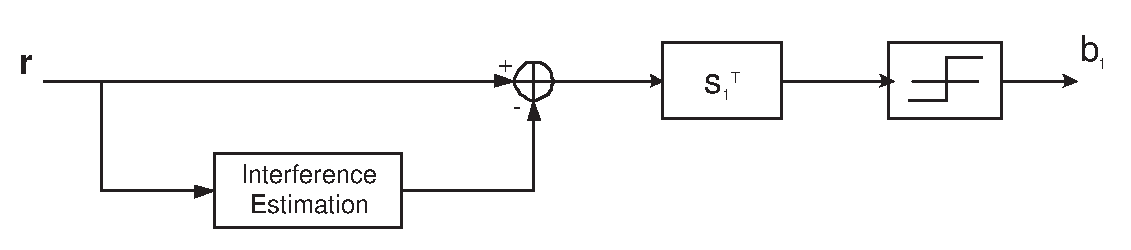
\includegraphics[width=6in]{IC_block.eps}}
\caption{The block structure of a basic interference cancellation
detector for user 1.} \label{IC}
\end{figure}

Interference cancellation is one of several multiuser detection
methods to suppress the effects from the MAI and consequently in
return increase the capacity of CDMA systems. As in figure
\ref{IC}, there are usually two basic stages in interference
cancellation realization. At the first stage, the MAI from other
users are reconstructed. At the second stage, the MAI is removed
from the received signal and the final decision is made from the
rest signal through a matched filter. Thus, the key part in
interference cancellation is how to estimate MAI as efficiently as
possible.

Without loss of the generality, assume only the bits $b_1$ sent by
the first user is considered in the following description. With
equation (\ref{r}), the received signature vector $\br$ can be
expressed as the combination of the desired signal vector, MAI and
AWGN vector as the following equation.

\begin{equation}
\begin{array}{rcl}
\br&=&b_1A_1\bs_1+\sum\limits_{k=2}^{K}b_k A_k\bs_k+\bn\\ &=&b_1
A_1\bs_1+\tilde{\bS}\tilde{\bA}\tilde{\bb}+\bn\\ &=&b_1
A_1\bs_1+\bm+\bn
\end{array}\label{rmn}
\end{equation}

\noindent where $\tilde{\bS}=[\matrix{\bs_2&\bs_3&\ldots&\bs_K}]$,
$\tilde{\bA}=diag\{\matrix{A_2&A_3&\ldots&A_K}\}$,
$\tilde{\bb}=[\matrix{b_2&b_3&\ldots&b_K}]^T$ and
\begin{equation}
\begin{array}{rcccl}
\bm&=&\sum\limits_{k=2}^{K}b_k
A_k\bs_k&=&\tilde{\bS}\tilde{\bA}\tilde{\bb}
\end{array}\label{m}
\end{equation}

\noindent denotes the MAI \footnote{Without loss of generality,
$\bm$ specially denotes the MAI to user 1 in this paper.}.

Before further discussion about interference cancellation, it will
be helpful to clarify the geometric meaning of single-user matched
filter. For this, the following proposition is presented.

\begin{Prop}

If $\hat\br_1$ is an observation of $b_1A_1\bs_1$, the output of
this observation through the single-user matched filter followed
by a limiter

\begin{equation}
\begin{array}{rcl}
\hat{b}_1&=&\mbox{sgn}\left\{\bs_1^T\hat\br_1\right\}
\end{array}
\end{equation}

\noindent actually is the solution to the following equation

\begin{equation}
\begin{array}{rcl}
\min\limits_{b}\left\|\hat\br_1-bA_1\bs_1\right\|_2&\mbox{subject
to}&b\in\{\pm1\}
\end{array}
\end{equation}

\noindent where $A_1$ denotes the unknown amplitude.

\end{Prop}

When the interference is estimated as $\hat{\bm}$, the output of
interference cancellation is the solution to the following
equation

\begin{equation}
\begin{array}{rcl}
\hat{b}_1=\mbox{arg}\min\limits_{b}\left\|\br-\hat{\bm}-bA_1\bs_1\right\|_2&\mbox{subject
to}&b\in\{\pm1\}
\end{array}\label{b-IC}
\end{equation}

\noindent and the result is

\begin{equation}
\begin{array}{rcl}
\hat{b}_1&=&\mbox{sgn}\left\{\bs_1^T(\br-\hat\bm)\right\}.
\end{array}
\end{equation}


In the following, how to the estimation of the MAI will be
presented in details with different criteria.

\subsection{Perfect Interference Cancellation}

In perfect interference cancellation (PEIC), the MAI is supposed
to be accurately estimated. Hence, with the equation (\ref{rmn}),
the estimated interference $\bm^{PEIC}$ for user 1 is

\begin{equation}
\begin{array}{rcl}
\bm^{PEIC}&=&\bm\hspace{0.1in}.
\end{array}
\end{equation}

In order to estimation $b_1$, the best strategy clearly is to
subtract $\bm$ from the received signal vector $\br$. The output
of perfect interference cancellation detector is

\begin{equation}
\begin{array}{rcccl}
b_1^{PEIC}&=&\mbox{sgn}\{\bs_1^T(\br-\bm^{PEIC})\}&=&\mbox{sgn}\{b_1+\bs_1^T\bn\}
\end{array}\hspace{0.1in}.
\end{equation}

Obviously, this result is the same to the single-user case with
AWGN channel.

\subsection{Individually Optimum Interference Cancellation}

In individually optimum interference cancellation (IO-IC), the
interference $\bm$ is estimated and removed from the observation
so that the optimum output $b_1^{IO}$ is expected to minimizes the
following error probability function

\begin{equation}
\begin{array}{rcl}
b_1^{IO}&=&\mbox{arg}\min\limits_{b}\ P[b\neq b_1]\\
&=&\mbox{arg}\min\limits_{b}\left\{\sum\limits_{\bd}P[b\neq b_1\
|\ \bd]P[\tilde{\bb}=\bd]\right\} \hspace{0.1in}.
\end{array}\label{b-IO}
\end{equation}

Due to the absolute value functions and alphabet combinations in
equation (\ref{b-IO}), it is very hard to give a close-form
solution to this kind of optimization problem. However, with the
following theorem, we can show that there does exist an possible
estimate of MAI $\hat{\bm}$ so that the output of interference
canceller can be is equal to $b_1^{IO}$.

\begin{lemma}
For any possible observation $\br$ as in equation (\ref{r}), there
exists a vector $\tilde{\bd}\in\{\pm 1\}^{(K-1)\times 1}$ so that
the output of individually optimum multiuser detection $b_1^{IO}$
is also the solution to the following equation

\begin{equation}
\begin{array}{rcl}
b_1^{IO}=\mbox{arg}\min\limits_{b}\left\|\br-\tilde{\bS}\tilde{\bA}\tilde{\bd}-bA_1\bs_1\right\|_2&\mbox{
subject to }& b\in\{\pm1\}\hspace{0.1in}.
\end{array}\label{m-IO}
\end{equation}
\label{IO-IC}\label{Lemma-IO}
\end{lemma}

\begin{proof}

Equation (\ref{b-IO}) can be expressed as

\begin{equation}
\begin{array}{rcl}
\mbox{arg}\min\limits_{b} P[b\neq
b_1]&=&\mbox{arg}\min\limits_{b}\left\{\sum\limits_{\bd}P[b\neq
b_1\ |\ \bd]P[\tilde{\bb}=\bd]\right\}\\
&=&\mbox{arg}\max\limits_{b}\left\{\sum\limits_{\bd}\exp\left\{-{2\over\sigma^2}\|\br-\tilde{\bS}\tilde{\bA}\bd-bA_1\bs_1\|_2^2\right\}P[\tilde{\bb}=\bd]\right\}
\hspace{0.1in}.
\end{array}
\end{equation}

Now there is the claim that, for any observation $\br$, if there
exists $b_1'\in\{\pm 1\}$, which satisfies the following function,


\begin{equation}
\begin{array}{rccl}
\left\|\br-\tilde{\bS}\tilde{\bA}\bd-b_1'A_1\bs_1\right\|_2&>&\left\|\br-\tilde{\bS}\tilde{\bA}\bd+b_1'A_1\bs_1\right\|_2\mbox{,}&\forall\
\bd\in\{\pm 1\}^{(K-1)\times 1}\hspace{0.1in},
\end{array}
\end{equation}

\noindent it will never be the optimum solution to equation
(\ref{b-IO}).

Hence, for any possible observation $\br$, there exist
$\hat{b}_1\in\{\pm 1\}$ and $\tilde{\bd}\in\{\pm 1\}^{(K-1)\times
1}$, which satisfy equation (\ref{b-IO}) and (\ref{m-IO}).
\end{proof}

With lemma \ref{IO-IC}, we show that the individually optimum
multiuser detection can be presented as an interference canceller.
At this time, the desired MAI estimation can be set to
$\bm^{IO}=\tilde{\bS}\tilde{\bA}\tilde{\bd}$ and the output of the
individually optimum interference cancellation is

\begin{equation}
\begin{array}{rcl}
b_1^{IO}&=&\mbox{sgn}\{\bs_1^T(\br-\bm^{IO})\}\\
&=&\mbox{sgn}\{b_1+\bs_1^T(\bm-\bm^{IO})+\bs_1^T\bn\}\hspace{0.1in}.
\end{array}\label{b-IO-IC}
\end{equation}

\subsection{Jointly Optimum Interference Cancellation}

Similar to the jointly optimum multiuser detector, it is expected
that the output of the jointly optimum interference cancellation
detector is the solution to the minimization of the following
joint error probability function

\begin{equation}
\begin{array}{rcl}
\bb^{JO}=\mbox{arg}\min\limits_{\bar{\bb}} P[\bar{\bb}\neq
\bb]&\mbox{subject to}&\bar{\bb}\in\{\pm 1\}^{K\times
1}\hspace{0.1in}.
\end{array}\label{b-JO}
\end{equation}

It is not easy to give a close-form solution to equation
(\ref{b-JO}) for interference cancellation, too. But, we can show
that the desired MAI estimate $\hat{\bm}$ for the jointly optimum
interference cancellation exists and can be estimated with the
following theorem.

\begin{lemma}
Suppose $\bb^{JO}=[b_1^{JO}\ (\tilde{\bb}^{JO})^T]^T \in\{\pm
1\}^{K\times 1}$ is the jointly optimum solution which minimizes
the joint error probability function as in equation (\ref{b-JO}).
If $\hat{\bm}$ is set to be
$\bm^{JO}=\tilde{\bS}\tilde{\bA}\tilde{\bb}^{JO}$, the output
$\hat{b}_1$ with equation (\ref{b-IC}) is equal to $b_1^{JO}$.
\label{Lemma-JO}
\end{lemma}

\begin{proof}
As we know, the vector $\bb^{JO}$ defined as in equation
(\ref{b-JO}) actually also is the optimum solution to the
following equation.

\begin{equation}
\begin{array}{rcl}
\bb^{JO}=\mbox{arg}\min\limits_{\bar{\bb}}\left\|\br-\bS\bA\bar{\bb}\right\|&\mbox{subject
to}&\bar{\bb}\in\{\pm 1\}^{K\times 1}\hspace{0.1in}.
\end{array}\label{b-JO2}
\end{equation}

At this time, with equation (\ref{b-IC}) and the MAI estimate
$\hat{\bm}=\tilde{\bS}\tilde{\bA}\tilde{\bb}^{JO}$, the output
$\hat{b}_1$ is the optimum solution to

\begin{equation}
\begin{array}{rcl}
\hat{b}_1=\mbox{arg}\min\limits_{b}\left\|\br-\tilde{\bS}\tilde{\bA}\tilde{\bb}^{JO}-bA_1\bs_1\right\|_2&\mbox{subject
to}&b\in\{+1,\ -1\}
\end{array}
\end{equation}

\end{proof}

With Lemma \ref{Lemma-JO}, it reveals that jointly optimum
multiuser detection can be realized as interference canceller. In
the jointly optimum interference cancellation, the key then is how
to optimally estimate the MAI $\bm^{JO}$. After the interference
$\bm^{JO}$ is estimated, the output of the jointly optimum
interference cancellation can be expressed as

\begin{equation}
\begin{array}{rcl}
b_1^{JO}&=&\mbox{sgn}\{\bs_1^T(\br-\bm^{JO})\}\\
&=&\mbox{sgn}\{b_1+\bs_1^T(\bm-\bm^{JO})+\bs_1^T\bn\}\hspace{0.1in}.
\end{array}\label{b-JO-IC}
\end{equation}

\subsection{Direct Interference Cancellation}

As we see, there are many optimum schemes proposed to estimate the
MAI $\bm$ with the known signature vectors $\bs_k$, $k=1$, $2$,
$\ldots$, $K$, and different criterion. Though these optimum
algorithms have very good performance, their computation usually
is so complex and depends not only on the decision rule but also
on the information vector alphabet. Hence, it is reasonable to
look for some suboptimum algorithms with low computation
complexity and good performance. In this section, another scheme
is proposed to estimate MAI $\bm$ directly with $\bS$. It is
expected that the estimated MAI $\hat{\bm}$ minimize the following
equation

\begin{equation}
\begin{array}{rcl}
\bm^{D-IC}&=&\mbox{arg}\min\limits_{\hat{\bm}}\left\|\hat{\bm}-(\br-b_1A_1\bs_1)\right\|_2\hspace{0.1in}.
\end{array}
\end{equation}

Before estimating the MAI $\bm$, a Household transformation $\bQ$
is defined to be performed on both sides of the equation (\ref{r})
so that

\begin{equation}
\begin{array}{rcccl}
\bQ^T\br&=&\bar{\br}&=&\left[\matrix{r_1\cr\bar{\br}_2}\right]
\end{array}\label{Qr}
\end{equation}

\noindent and

\begin{equation}
\begin{array}{rcccl}
\bQ^T\bS&=&\bQ^T[\matrix{\bs_1&\tilde{\bS}}]&=&\left[\matrix{c&\bar{\bs}_{21}^T\cr\mathbf{0}&\tilde{\bS}_{22}}\right]
\end{array}\label{QS}
\end{equation}

\noindent where $r_1$ is the first element in the vector
$\bar{\br}$, $\bar{\br}_2$ is the $(L-1)\times 1$ complement
subvector of $r_1$, $\bar{\bs}_{21}$ is a $(K-1)\times 1$ vector
and $\tilde{\bS}_{22}$ is a $(L-1)\times (K-1)$ matrix and
$c=\pm\|\bs_1\|_2=\pm1$. This Household transformation can then be
written as

\begin{equation}
\begin{array}{rcccl}
\bQ&=&\bI-2\bq\bq^T&=&\bI-{1\over
c(c-s_{11})}\left[\matrix{(s_{11}-c)\cr s_{12}\cr\vdots\cr
s_{1L}}\right]\left[\matrix{(s_{11}-c)&s_{12}&\cdots&s_{1L}}\right]
\end{array}
\end{equation}

\noindent where
$\bq={1\over\sqrt{2c(c-s_{11})}}\left[\matrix{(s_{11}-c)&s_{12}&\cdots&s_{1L}}\right]^T$
and $s_{11}$ is the first element of $\bs_1$.


Now, the direct estimation of the MAI $\bm$ can be realization
with the following lemma.

\begin{lemma} The minimum norm (or least squares )solutions to the
following equation

\begin{equation}
\begin{array}{rcl}
\bx&=&\matrix{\mbox{arg}\min\limits_{\bx}\left\|\tilde{\bS}\bx-(\br-b_1A_1\bs_1)\right\|_2}
\end{array}
\end{equation}

\noindent is given by

\begin{equation}
\begin{array}{rcl}
\bx&=&\tilde{\bS}_{22}^+\bar{\br}_2
\end{array}
\end{equation}
\end{lemma}

Before proving the above theorem, we introduce the following
conclusion.

\begin{Prop}

\begin{equation}
\begin{array}{rcl}
\left[\matrix{c&\bar{\bs}_{21}^T\cr\mathbf{0}&\tilde{\bS}_{22}}\right]^+&=&\left[\matrix{\frac{1}{c}&-\frac{1}{c}\bar{\bs}_{21}^T\tilde{\bS}_{22}^+\cr\mathbf{0}&\tilde{\bS}_{22}^+}\right]\end{array}
\end{equation}
\end{Prop}

\begin{proof}
We know that
\begin{equation}
\begin{array}{rcl}
\tilde{\bS}\bx-(\br-b_1A_1\bs_1)&=&\bS\left[\matrix{b_1A_1\cr\bx}\right]-\br\\
&=&\left[\matrix{c&\bar{\bs}_{21}^T\cr\mathbf{0}&\tilde{\bS}_{22}}\right]\left[\matrix{b_1A_1\cr\bx}\right]-\left[\matrix{r_1\cr\bar{\br}_2}\right]
\end{array}
\end{equation}

\noindent Then,

\begin{equation}
\begin{array}{rcl}
\mbox{arg}\min\limits_{\bx}\left\|\tilde{\bS}\bx-(\br-b_1A_1\bs_1)\right\|&=&\mbox{arg}\min\limits_{\bx}\left\|\left[\matrix{c&\bar{\bs}_{21}^T\cr\mathbf{0}&\tilde{\bS}_{22}}\right]\left[\matrix{b_1A_1\cr\bx}\right]-\left[\matrix{r_1\cr\bar{\br}_2}\right]\right\|\\
&=&\mbox{arg}\min\limits_{\bx}\left\|\left[\matrix{b_1A_1\cr\bx}\right]-\left[\matrix{\frac{1}{c}&-\frac{1}{c}\bar{\bs}_{21}^T\tilde{\bS}_{22}^+\cr\mathbf{0}&\tilde{\bS}_{22}^+}\right]\left[\matrix{r_1\cr\bar{\br}_2}\right]\right\|\\
&=&\mbox{arg}\min\limits_{\bx}\left\|\left[\matrix{b_1A_1\cr\bx}\right]-\left[\matrix{\frac{r_1}{c}-\frac{1}{c}\bar{\bs}_{21}^T\tilde{\bS}_{22}^+\bar{\br}_2\cr\tilde{\bS}_{22}^+\bar{\br}_2}\right]\right\|
\end{array}
\end{equation}

\noindent Thus,

\begin{equation}
\begin{array}{rcl}
\mbox{arg}\min\limits_{\bx}\left\|\tilde{\bS}\bx-(\br-b_1A_1\bs_1)\right\|&=&\tilde{\bS}_{22}^+\bar{\br}_2
\end{array}
\end{equation}


\end{proof}

Hence, the estimation of $\bm$ with the minimum norm estimation of
the vector $\tilde{\bA}\tilde{\bb}$ is

\begin{equation}
\begin{array}{rcl}
\bm^{D-IC}&=&\tilde{\bS}\tilde{\bS}_{22}^+\bar{\br}_2
\end{array}\label{m-DIC}
\end{equation}

After the interference is estimated, it can be removed out from
the received signal. Thus, the output of the proposed direct
interference cancellation detector is

\begin{equation}
\begin{array}{rcl}
b_1^{D-IC}&=&\mbox{sgn}\left\{\bs_1^T
\left(\bI_L-\tilde{\bS}\tilde{\bS}_{22}^{+}\left[\matrix{\mathbf{0}&\bI_{(L-1)}}\right]\bQ^T\right)\br\right\}
\end{array} \label{b_IC}
\end{equation}

\noindent where $\bI_{L}$ is a $L\times L$ identity matrix and
$\bI_{L-1}$ is a $(L-1)\times (L-1)$ identity matrix.

Thus, the linear filter representation of the direct interference
cancellation detector is

\begin{equation}
\begin{array}{rcl}
\bw_1^{D-IC}&=&\left(\bI_L-\bQ\left[\matrix{\mathbf{0}^T\cr\bI_{(L-1)}}\right]\tilde{\bS}_{22}^{+T}\tilde{\bS}^T\right)\bs_1
\end{array} \hspace{0.1in}. \label{w_IC}
\end{equation}

\subsection{Maximum Asymptotic Multiuser Efficiency Interference Cancellation}

As we know, the effective energy of user 1 $e_1(\sigma)$ is always
upper bounded by the actual energy $A_1^2$. Multiuser efficiency
or ratio between the effective energy and actual energy,
$e_1(\sigma)/A_1^2$, which depends on the signature waveforms,
received signal-to-noise ratio (SNR) and the employed detector, is
always not larger than 1. The asymptotic multiuser efficiency
(AME) for user $1$ is defined as


\begin{equation}
\begin{array}{rcl}
\eta_1&=&\lim\limits_{\sigma\rightarrow0}{e_1(\sigma)\over
A_1^2}\hspace{0.1in},
\end{array}\label{AME}
\end{equation}

\noindent which measure the slope when user 1's error probability


\begin{equation}
\begin{array}{rcl}
P_{e1}&=&Q\left({e_1(\sigma)\over \sigma}\right)
\end{array}\label{BER}
\end{equation}

\noindent in logarithmic scale goes to 0 in the high SNR region.

Now, we discuss the linear transformation which can maximize the
possible asymptotic multiuser efficiency. We denote the linear
transformation for MAI estimation in MAME interference
cancellation by $\bW_{1}^{m}$ so that

\begin{equation}
\begin{array}{rcl}
\bW_{1}^{mT}\br&=&\bm^{MAME-IC}
\end{array}
\end{equation}

The the error probability achieve by $\bW_{1}^{m}$ and $\bs_1$ can
be expressed as

\begin{equation}
\begin{array}{rcl}
P_{e1}&=&\mbox{E}\left[Q\left({\bs_1^T\br-\bs_1^T\bW_{1}^{mT}\br\over
\sigma\|\bs_1-\bW_{1}^{m}\bs_1\|_2}\right)\right]\\
&=&\mbox{E}\left[Q\left({A_1b_1+\sum\limits_{k=2}^{K}A_kb_k\rho_{1k}-\sum\limits_{k=1}^KA_kb_k\bw_{1}^{mT}\bs_k\over
\sigma\|\bs_1-\bw_{1}^{m}\|_2}\right)\right]
\end{array}\label{b-Q}
\end{equation}

\noindent Where $\bw_{1}^{m}=\bW_{1}^{m}\bs_1$ and the expectation
is with respect to $b_j$, $j\neq 1$. The asymptotic multiuser
efficiency of user 1 is given by the square of the smallest
argument in equation (\ref{b-Q}) normalized by $A_1^2/\sigma^2$

\begin{equation}
\begin{array}{rcl}
\eta_1(\bw_{1}^{m})&=&\max^2\left\{\matrix{0,{1\over\|\bs_1-\bw_{1}^{m}\|_2}\left(1-\bs_1^T\bw_{1}^{m}-\sum\limits_{k=2}^{K}{A_k\over
A_1}\left|\rho_{1k}-\bs_k^T\bw_{1}^{m}\right|\right)}\right\}\hspace{0.01in}.
\end{array}\label{MAME-IC}
\end{equation}


As the MAME linear multiuser detector~\cite{Lupa89}, due to the
presence of the absolute value function in equation
(\ref{MAME-IC}), solve this optimization problem for $K$-user case
doesn't admit a closed-form solution.

After the estimation of the interference $\bm^{MAME-IC}$, it is
removed from the observation $\br$ and the output of the MAME
interference cancellation is

\begin{equation}
\begin{array}{rcl}
b_1^{MAME-IC}&=&\mbox{sgn}\{\bs_1^T(\br-\bm^{MAME-IC})\}\\
&=&\mbox{sgn}\{b_1+\bs_1^T(\bm-\bm^{MAME-IC})+\bs_1^T\bn\}\hspace{0.1in}.
\end{array}
\end{equation}

\subsubsection{Two-user Case}
When there are only two active users, equation (\ref{MAME-IC}) can
be simplified as

\begin{equation}
\begin{array}{rcl}
\eta_1&=&\max^2\left\{\matrix{0,{1\over\|\bs_1-\bw_{1}^{m}\|_2}\left(1-\bs_1^T\bw_{1}^{m}-{A_2\over
A_1}\left|\rho-\bs_2^T\bw_{1}^{m}\right|\right)}\right\}\hspace{0.01in},
\end{array}\label{MAME-IC2}
\end{equation}

\noindent where $\bw_1^m$ is a linear combination of $\bs_1$ and
$\bs_2$.

Solving equation (\ref{MAME-IC2}) can lead to the following
solution.

\begin{equation}
\begin{array}{rcl}
\bw_{1}^{m}&=&\left\{\begin{array}{ll}{A_1\over
A_2}\mbox{sgn}(\rho)\bs_2 ,&\mbox{if }{A_2\over A_1}<|\rho| ,\\
\rho\bs_2 ,&\mbox{otherwise.}\end{array}\right.
\end{array}
\end{equation}

Compared to the MAME detector for user $1$,

\begin{equation}
\begin{array}{rcl}
\bw_1&=&\left\{\begin{array}{ll}\bs_1-{A_1\over
A_2}\mbox{sgn}(\rho)\bs_2,&\mbox{if }{A_2\over A_1}<|\rho|,\\
\bs_1-\rho\bs_2 ,&\mbox{otherwise, }\end{array}\right.
\end{array}
\end{equation}

\noindent we can see that they are actually identical one.

\subsection{Minimum Mean-Square Error Interference Cancellation}

In this section, we are going to propose a minimum mean-square
error interference cancellation (MMSE-IC) scheme, in which the MAI
is estimated with minimizing the output variance as in the
following function

\begin{equation}
\begin{array}{rcl}
\bm^{MMSE-IC}&=&\mbox{arg}\min\limits_{\hat{\bm}_{n}}\
E\left\{[\bs_1^T(\br-b_1A_1\bs_1)-\bs_1^T\hat{\bm}]^2\right\}
\hspace{0.1in}.
\end{array}\label{m_MMSE}
\end{equation}

Hence, the output of the MMSE interference cancellation can be
written as

\begin{equation}
\begin{array}{rcl}
b_1^{MMSE-IC}&=&\mbox{sgn}\{\bs_1^T(\br-\bm^{MMSE})\}\\
&=&\mbox{sgn}\{b_1+\bs_1^T(\bm-\bm^{MMSE})+\bs_1^T\bn\}\hspace{0.1in}.
\end{array}
\end{equation}

One possible linear solutions to equation (\ref{m_MMSE}) is to
estimate

\begin{equation}
\begin{array}{rcl}
\bm^{MMSE-IC}=\bs_1\bar\bw^T\br&\mbox{with}&\bar\bw=\mbox{arg}\min\limits_{\hat\bw}\
E\left\{[\bs_1^T(\br-b_1A_1\bs_1)-\hat\bw^T\br]^2\right\}
\end{array}\label{LMMSE}
\end{equation}

The close-form solution to the equation (\ref{LMMSE}) can be
presented in the following theorem.

\begin{lemma} The solution to

\begin{equation}
\begin{array}{rcl}
\bar\bw&=&\mbox{arg}\min\limits_{\hat\bw}\
E\left\{[\bs_1^T(\br-b_1A_1\bs_1)-\hat\bw^T\br]^2\right\}
\end{array}
\end{equation}

\noindent is

\begin{equation}
\begin{array}{rcl}
\bar\bw&=&(\bS\bA^2\bS^T+\sigma^2\bI_L)^{-1}(\tilde{\bS}\tilde{\bA}^2\tilde{\bS}^T+\sigma^2\bI_L)\bs_1
\end{array}
\end{equation}

\end{lemma}

\begin{proof}

It is easy to verify the following conclusion.

\begin{equation}
\begin{array}{rcl}
(\bS\bA^2\bS^T+\sigma^2\bI_L)^{-1}(\tilde{\bS}\tilde{\bA}^2\tilde{\bS}^T+\sigma^2\bI_L)&=&\mbox{arg}\min\limits_{\hat\bW}\
E\left\|(\br-b_1A_1\bs_1)-\hat\bW^T\br\right\|_2
\end{array}
\end{equation}

\noindent Then,

\begin{equation}
\begin{array}{rcl}
\bar\bw&=&(\bS\bA^2\bS^T+\sigma^2\bI_L)^{-1}(\tilde{\bS}\tilde{\bA}^2\tilde{\bS}^T+\sigma^2\bI_L)\bs_1
\end{array}
\end{equation}

\end{proof}

Thus, the output of the proposed linear MMSE interference
cancellation detector is

\begin{equation}
\begin{array}{rcl}
b_1^{MMSE-IC}&=&\mbox{sgn}\left\{\bs_1^T
\left[\bI_L-(\tilde{\bS}\tilde{\bA}^2\tilde{\bS}^T+\sigma^2\bI_L)(\bS\bA^2\bS^T+\sigma^2\bI_L)^{-1}\right]\br\right\}
\end{array}
\end{equation}

\noindent and the linear filter representation of the linear MMSE
interference cancellation detector is

\begin{equation}
\begin{array}{rcl}
\bw_1^{MMSE-IC}&=&\left[\bI_L-(\bS\bA^2\bS^T+\sigma^2\bI_L)^{-1}(\tilde{\bS}\tilde{\bA}^2\tilde{\bS}^T+\sigma^2\bI_L)\right]\bs_1\\
&=&A_1^2(\bS\bA^2\bS^T+\sigma^2\bI_L)^{-1}\bs_1 \hspace{0.1in}.
\end{array}\label{w_MMSEIC}
\end{equation}


\section{Performance Analysis}

As we see, in interference cancellation, After the MAI is
estimated and removed from the received signal, the decision is
simply made by projecting the rest signal vector onto the
signature vector of the desired user. Hence, the key is the
interference estimation in the first stage and the second stage is
fixed. Different MAI estimation schemes lead to different
interference cancellation algorithms. In the following, the
proposed interference cancellation detection schemes would be
compared with other multiuser detection algorithms.

In the perfect interference cancellation, the MAI is completely
removed with some help so that the result is same to that of the
optimally demodulating the signal, which is sent through a
single-user channel. Obviously, the performance of EIC is same to
that of the optimal receiver for the single-user channel and its
BER is

\begin{equation}
\begin{array}{rcl}
P_{e1}^{PEIC}&=&Q\left({A_1 \over \sigma}\right) \hspace{0.1in}.
\end{array}
\end{equation}

Obviously, the BER performance of the perfect interference
cancellation is the best we can obtain through the multiuser
channel with the assumption that the MAI is known. And its
asymptotic efficiency is always kept as $1$, which are are better
than any other multiuser scheme, since the MAI can be perfectly
removed from the received signal vector. Thus, the perfect
interference cancellation can be taken as the lowest bound for all
the possible multiuser detection schemes.

In the individually or jointly optimum interference cancellation,
the interference is estimated and cancelled so that the output of
the matched filter is a optimum solution to minimize the
individual or joint error probability function as in equations
(\ref{b-IO}) and (\ref{b-JO}), respectively. These two definitions
sound basically the same to that of the individually and jointly
optimum multiuser detection, respectively. Furthermore with Lemma
\ref{Lemma-IO} and \ref{Lemma-JO}, the optimum interference
cancellations can be taken the special realization of the optimum
multiuser detections, respectively. Hence, the performance of the
individually or jointly optimum interference cancellation can
achieve the same performance of the individually or jointly
optimum multiuser detection scheme, respectively.

In decorrelating detection, the receiver signal passes the
single-user matched filter first. The decorrelating operation then
is performed on the output. The final results are obtained with
limiters. The basic structure for decorrelating detection can be
shown in figure \ref{DD_block}. Compared with figure
\ref{DirectIC_block}, we can see that this is different to direct
inference cancellation. However, though decorrelating detection
and direct interference cancellation have different operation
structure, with the following lemma, we can see that the
decorrelating detector and the proposed direct interference
cancellation have the same performance. The proposed interference
cancellation then can be taken as a special realization of the
decorrelating detection.

\begin{figure}
\center{
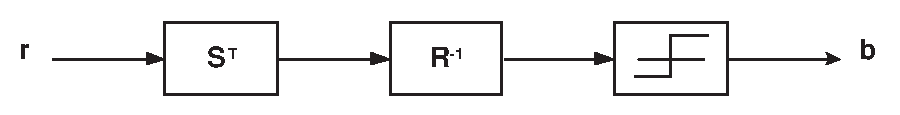
\includegraphics[width=4in]{DD_block_K.eps}}
\caption{The structure of decorrelating detector.}
\label{DD_block}
\end{figure}

\begin{figure}
\center{
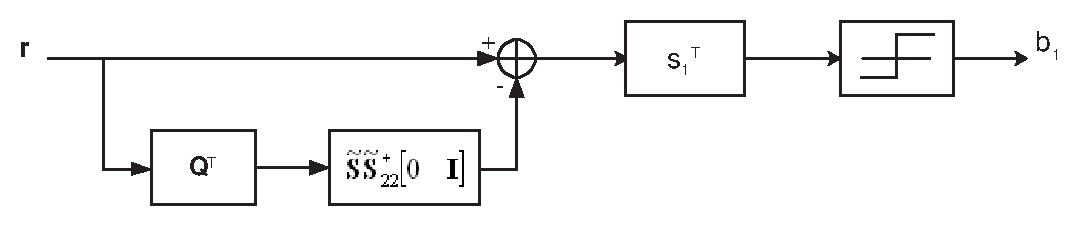
\includegraphics[width=4.5in]{DirectIC_block_K.eps}}
\caption{The structure of direct interference cancellation for
user 1} \label{DirectIC_block}
\end{figure}


\begin{lemma}
$\bw_1^{D-IC}=\alpha\bw_1^{DD}$, where $\alpha$ is a positive
factor, so that the proposed direct interference cancellation
detector has the same performance as that of the classic
decorrelating detector.\label{D-IC}
\end{lemma}
\begin{proof}
With the unitary transformation $\bQ$ on both sides of the
equation (\ref{r}), we got

\begin{equation}
\begin{array}{rcl}
\bQ^T\br&=&\left[\matrix{c&\bar{\bs}_{21}^T\cr\mathbf{0}&\tilde{\bS}_{22}}\right]\bA\bb+\bQ^T\bn
\end{array}\hspace{0.1in}.
\end{equation}
\noindent So that, as the same to the decorrelating detection, the
least-square estimation of $\bA\bb$ is
\begin{equation}
\begin{array}{rcl}
\bA\bb&=&\left[\matrix{c&\bar{\bs}_{21}^T\cr\mathbf{0}&\tilde{\bS}_{22}}\right]^+\bQ^T\br
\end{array}\hspace{0.1in}.
\end{equation}

Hence, the decorrelation detector can be written in the
interference cancellation form as
\begin{equation}
\begin{array}{rcl}
b_1^{DD}&=&\mbox{sgn}\left\{\left[\matrix{c^{-1}&-c^{-1}\bar{\bs}_{21}^T\tilde{\bS}_{22}^{+}}\right]\bQ^T\br\right\}
\end{array} \hspace{0.1in}.
\end{equation}

On the other hand, with equation (\ref{b_IC}), the output of the
interference detection detector is

\begin{equation}
\begin{array}{rcl}
b_1^{D-IC}&=&\mbox{sgn}\left\{\bs_1^T
\left(\bI_L-\tilde{\bS}\tilde{\bS}_{22}^{+}\left[\matrix{\mathbf{0}&\bI_{(L-1)}}\right]\bQ^T\right)\br\right\}\\
&=&\mbox{sgn}\left\{\left([\matrix{c&0&\ldots&0}]-[\matrix{c&0&\ldots&0}]\left[\matrix{\bar{\bs}_{21}\cr\tilde{\bS}_{22}}\right]\left[\matrix{\mathbf{0}&\tilde{\bS}_{22}^{+}}\right]\right)\bQ^T\br\right\}\\
&=&\mbox{sgn}\left\{\left[\matrix{c&-c\bar{\bs}_{21}^T\tilde{\bS}_{22}^{+}}\right]\bQ^T\br\right\}
\hspace{0.1in}.
\end{array}
\end{equation}

Thus, $\bw_1^{D-IC}=c^2\bw_1^{DD}$ and the proposed interference
cancellation detector has the same performance as that of the
classic decorrelating detector.
\end{proof}

As we know, with decorrelating detector, the received signal
vector $\br$ is projected on the subspace orthogonal to the codes
of the other users~\cite{Verd98,Tse99}. It is shown
in~\cite{Elda02} that the decorrelating detector is the {\em
oblique projection} of the desired user's signature vector onto
the space $\underline{\mathbf{\cal S}}_1$, which is the orthogonal
complement of subspace spanned by other users' signature vectors,
along $\mathbf{\cal S}_1$ the orthogonal complement space of this
space. For example, the decorrelating detector $\bw_{1}^{DD}$ for
the first user is

\begin{equation}
\begin{array}{rcl}
\bw_{1}^{DD}&=&\bP_1^{O}\bs_1\\
 &=&{1 \over \bs_1^H\bP_1^{\perp}\bs_1 }\bP_1^{\perp}\bs_1
\end{array}
\end{equation}

\noindent where

\begin{equation}
\begin{array}{rcl}
\bP_1^{O}\bs_1&=&{1 \over \bs_1^H\bP_1^{\perp}\bs_1
}\bP_1^{\perp}\bs_1\bs_1^H
\end{array}
\end{equation}

\noindent denotes the oblique projection of $\bs_1$, and
$\bP_1^{\perp}$ is the orthogonal projection for user 1 onto the
orthogonal complement of the space spanned by the other users'
signature vectors. This can be demonstrated on figure \ref{DD}.

\begin{figure}
\center{
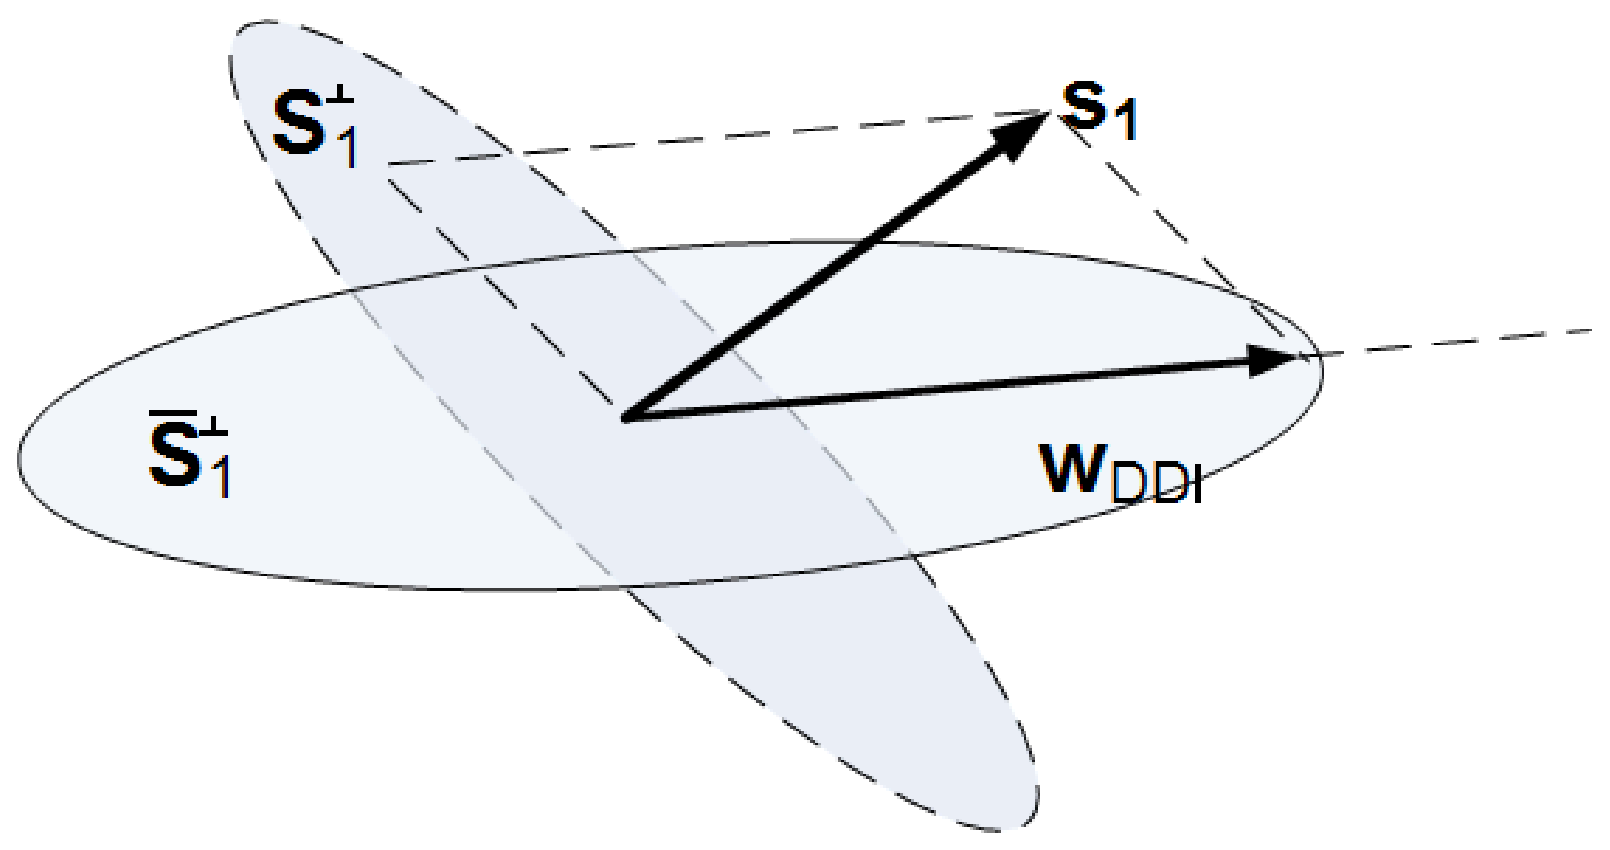
\includegraphics[width=3in]{DD_geometric.eps}}
\caption{The geometric demonstration of the decorrelating detector
for user 1.} \label{DD}
\end{figure}

Different to the decorrelating multiuser detection, the output of
the direct interference cancellation is the result of the
different between the observation $\br$ and the MAI $\bm^{D-IC}$.
Hence, the linear filter representation of direct interference
cancellation can actually be take as the difference between
$\bs_1$ and $\bw_{m1}^{D-IC}$ as in equation (\ref{w_IC}), where
$\bw_{m1}^{D-IC}$ is the linear filter representation of the MAI
estimation in the direct interference cancellation and can be
expressed as

\begin{equation}
\begin{array}{rcl}
\bw_{m1}^{D-IC}&=&\bQ\left[\matrix{\mathbf{0}^T\cr\bI_{(L-1)}}\right]\tilde{\bS}_{22}^{+T}\tilde{\bS}^T\bs_1
\end{array} \hspace{0.1in}.
\end{equation}

Furthermore, with the definition of $\bm$ as in equation
(\ref{m}), $\bw_{m1}^{D-IC}$ belongs to the linear subspace
$\mathbf{\cal S}_{m1}$ spanned by other signature vectors. Thus,
the linear filter representation of the direct interference
cancellation can be taken the oblique projection of $\bs_1$ on to
$\underline{\mathbf{\cal S}}_1$ along $-\bw_{m1}^{D-IC}$. This can
be demonstrated in figure \ref{DIC}


\begin{figure}
\center{
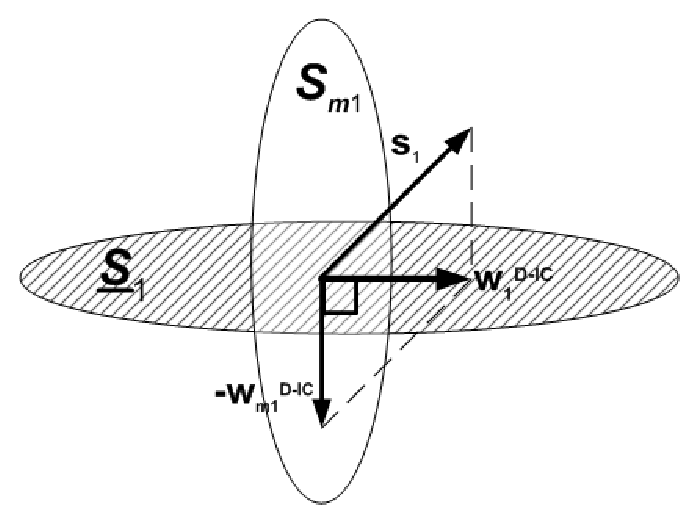
\includegraphics[width=3in]{DirectIC_geometric.eps}}
\caption{The geometric demonstration of the direct interference
cancellation for user 1.} \label{DIC}
\end{figure}


Based on the definition of the $\bm^{MAME-IC}$, it can be take as
the combination of the single-user matched filter and the
direction interference cancellation. The basic structure for
tow-user MAME multiuser detection and MAME interference
cancellation are shown in figure \ref{MAME_block} and
\ref{MAMEIC_block}, respectively. With Lemma \ref{D-IC}, the
performance of the proposed MAME interference cancellation
detector obviously is same to that of the MAME multiuser detector.

\begin{figure}
\center{
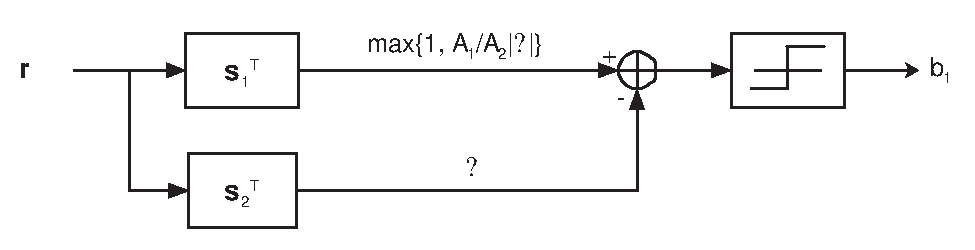
\includegraphics[width=4in]{MAME_block.eps}}
\caption{The structure of two-user MAME detector for user 1.}
\label{MAME_block}
\end{figure}

\begin{figure}
\center{
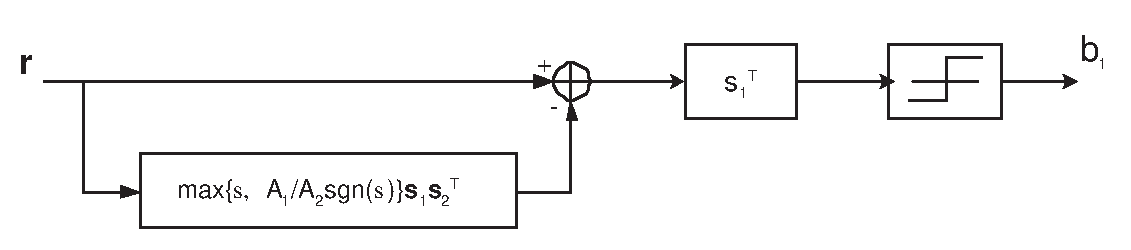
\includegraphics[width=4.5in]{MAMEIC_block.eps}}
\caption{The structure of two-user MAME interference cancellation
for user 1} \label{MAMEIC_block}
\end{figure}


The classic linear MMSE detector can be seen as a compromise
solution that takes into account the relative importance of each
interfering user and the background noise. The basic structure for
MMSE detector is shown in figure \ref{MMSE_block}. Obviously, it
is different to the structure of MMSE interference cancellation,
which is shown in figure \ref{MMSEIC_block}. With the following
theorem, we can see that the proposed linear MMSE interference
cancellation detector and the classic linear MMSE detector are
also of the same performance.


\begin{figure}
\center{
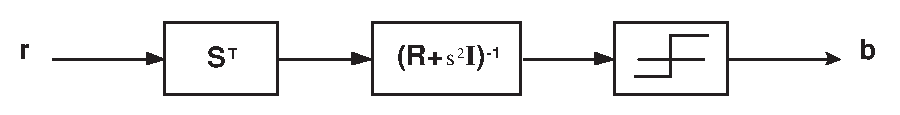
\includegraphics[width=4in]{MMSE_block_K.eps}}
\caption{The structure of MMSE detector.} \label{MMSE_block}
\end{figure}

\begin{figure}
\center{
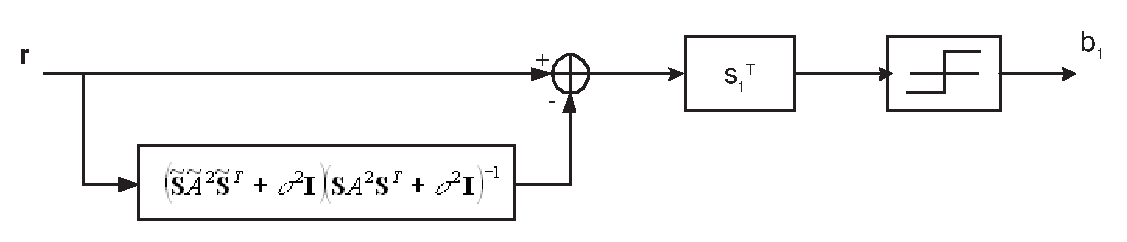
\includegraphics[width=4.5in]{MMSEIC_block_K.eps}}
\caption{The structure of MMSE interference cancellation for user
1} \label{MMSEIC_block}
\end{figure}

\begin{Prop}
There is the following relationship.
\begin{equation}
\begin{array}{rcl}
(\bS\bA^2\bS^T+\sigma^2\bI_L)^{-1}\bS\bA^2&=&\bS(\bS^T\bS+\sigma^2\bA^{-2})^{-1}
\end{array}
\end{equation}\label{p1}
\end{Prop}
\begin{proof}
It easy to see the following relationship.
\begin{equation}
\begin{array}{rcccl}
\bS\bA^2\bS^T\bS+\sigma^2\bS&=&\bS\bA^2(\bS^T\bS+\sigma^2\bA^{-2})\\
&=&(\bS\bA^2\bS^T+\sigma^2\bI_L)\bS\hspace{0.1in}.
\end{array}
\end{equation}
Thus,
\begin{equation}
\begin{array}{rcl}
(\bS\bA^2\bS^T+\sigma^2\bI_L)^{-1}\bS\bA^2&=&\bS(\bS^T\bS+\sigma^2\bA^{-2})^{-1}
\end{array}
\end{equation}
\end{proof}

\begin{lemma} $\bw_1^{MMSE-IC}=\beta\bw_1^{MMSE}$, where $\beta$ is a positive
factor, so that the proposed MMSE interference cancellation
detector has the same performance as the classic MMSE multiuser
detector.
\end{lemma}
\begin{proof}
As we know, the linear filter representation of the MMSE multiuser
detector for user 1 is
\begin{equation}
\begin{array}{rcl}
\bw_1^{MMSE}&=&\bS(\bS^T\bS+\sigma^2\bA^{-2})^{-1}\be_1\hspace{0.1in},
\end{array}
\end{equation}
\noindent where $\be_1=[\matrix{1&0&\ldots&0}]^T$ is a $K\times 1$
vector.

With Proposition \ref{p1},
\begin{equation}
\begin{array}{rcl}
\bw_1^{MMSE-IC}&=&A_1^2\bw_1^{MMSE}\hspace{0.1in}.
\end{array}
\end{equation}
\end{proof}


\section{Conclusions}

In this paper, the principles of the interference detection is
reviewed. Besides individually and jointly optimum interference
cancellation, direct interference cancellation, MAME interference
cancellation and MMSE interference cancellation are proposed. With
theoretical analysis, the optimum multiuser detectors can be
realized as interference cancellation. the performance of direct
interference cancellation, MAME interference cancellation and MMSE
interference cancellation are same to that of the decorrelating
detection, MAME multiuser detector and linear MMSE detector,
respectively.

\bibliographystyle{unsrt}
\bibliography{InterferenceCancellation}
\end{document}
